\documentclass[]{report}

\voffset=-1.5cm
\oddsidemargin=0.0cm
\textwidth = 480pt

\usepackage{framed}
\usepackage{subfiles}
\usepackage{graphics}
\usepackage{newlfont}
\usepackage{eurosym}
\usepackage{amsmath,amsthm,amsfonts}
\usepackage{amsmath}
\usepackage{enumerate}
\usepackage{color}
\usepackage{multicol}
\usepackage{amssymb}
\usepackage{multicol}
\usepackage[dvipsnames]{xcolor}
\usepackage{graphicx}
\begin{document}

% \maketitle

\section*{ Network analysis - introduction and terminology }
Objectives 1. After studying this chapter you will 
\begin{itemize}
\item  have been introduced to the control and planning technique called Network Analysis \item  know what is meant by; Activity, Event and Dummy Activity \item  understand the key rules for drawing Networks \item  know the various ways Activities are identified \item  be able to use Dummy Activities correctly. 
\end{itemize}
\subsection{Definition} 2. Network analysis is a generic term for a family of related techniques developed to aid management to plan and control projects. These techniques show the inter-relationship of the various jobs or tasks which make up the overall project and clearly identify the crit-ical parts of the project. They can provide planning and control information on the time, cost and resource aspects of a project. Network analysis is likely to be of most value where projects are: a) Complex, i.e. they contain many related and interdependent activities, and/or b) Large, i.e. where many types of facilities, high capital investments, many personnel are involved; and c) Where restrictions exists, i.e. where projects have to be completed within stipulated time or cost limits, or where some or all of the resources (material, labour) are limited. 
\subsection{Background} 3. A basic form of network analysis was being used in the UK and USA in the mid-1950's in an attempt to reduce project times. 
In 1958 the US Naval Special Projects Office set up a team to devise a technique to contro the planning of complex projects. 
The outcome of the team's efforts was the developm of the network technique known as PERT (Programme Evaluation and Review Technique). 
Pert was used to plan and control the development of the Polaris missile and w.. credited with saving two years in the missile's development. 
Since 1958 the technique has been developed and nowadays many variants exist w handle, in addition to basic time factors, costs, resources, probabilities and 
combina of all these factors. A variety of names exist and some of the more commonly used are

\begin{itemize}
	\item Critical Path Planning CPP 
	\item Critical Path Analysis CPA 
	\item Critical Path Scheduling CPS 
	\item Critical Path Method CPM 
	\item Programme Evaluation and Review Technique etc. PERT, PERT/COST 
\end{itemize} 

% 322 


%==================%



\subsection*{Basic network terminology}
Only the basic elements of networks are covered to start with, other more complex features are introduced as required in later chapters. 
\begin{itemize}
	\item 
\textbf{Activity} This is a task or job of work which takes time and resources e.g. Build a Wall, Verify the debtors in a sales ledger, Dig foundations etc. 

An activity is represented in a network by an arrow thus: 
\begin{figure}[h!]
\centering

\includegraphics[width=0.15\linewidth]{323-a}
% \caption{}
% \label{fig:323-a}
\end{figure}

The head of the arrow indicates where the task ends and the tail where the tasks begins. The arrow points from left to right but is not drawn to scale. An essential preliminary to the use of network analysis is establishing. a) what activities are involved in the project. b) their logical relationship e.g. the activity of Building a Wall must take place after the activity, Dig Foundations. c) an estimate of the time the activity is expected to take. Note that the basic time esti-mate is always necessary but in addition other estimates of times, costs, resources, probabilities etc may also be required. These other factors are dealt with later. 
\item \textbf{Event} This is a point in time and indicates the start or finish of an activity, or activities, e.g. Wall built, Debtors verified, Foundations Dug etc. An event is represented in a network by a circle or node thus: \begin{figure}[h!]
\centering

\includegraphics[width=0.1\linewidth]{323-b}
%\caption{}
%\label{fig:323-b}
\end{figure}

It will be noted that the establishment of activities automatically determines events because they are the start and finish of activities and represent the achievement of a specific stage of a project. 

\item \textbf{Dummy activity} This is an activity which does not consume time or resources. It is used merely to show clear, logical dependencies between activities so as not to violate the rules for drawing networks. It is represented on a network by a dotted arrow thus: =
\begin{figure}[h!]
\centering

\includegraphics[width=0.1\linewidth]{323-c}
% \caption{}
% \label{fig:323-c}
\end{figure}
 * Note that dummy activities are not usually listed with the real activities but become necessary as the network is drawn. Dummy activity examples are given after the rules for drawing networks have been discussed. 
\item \textbf{Network} This is the combination of activities, dummy activities and events in logical sequence according to the rules for drawing networks. Thus a small network might appear as follows: 

\end{itemize}
% 323 
\begin{figure}
\centering
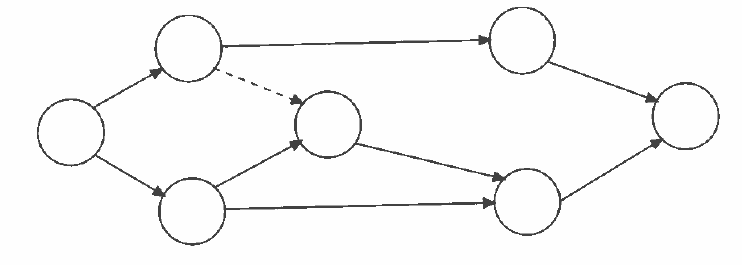
\includegraphics[width=0.4\linewidth]{324-a}
\caption{}
\label{fig:324-a}
\end{figure}


%=================%
\newpage
\subsection*{Rules for drawing networks}
 The following rules are all logically based and should be thoroughly learned before attempting to draw networks. 
\begin{itemize}
\item[(a)] 
A complete network should have only one point of entry - a start event and only one point of exit - a finish event. 
\item[(b)]  Every activity must have one preceding or 'tail'event and one succeeding or 'head' event. Note that many activities may use the same tail event and many may use the head event, e.g. 


\begin{figure}[h!]
\centering
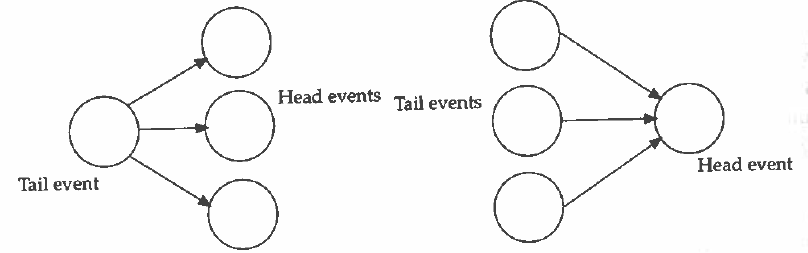
\includegraphics[width=0.4\linewidth]{324-b}
\caption{}
\label{fig:324-b}
\end{figure}


However an activity must not share the same tail event and the same head event with any other activities (this is dealt with in detail in Para 8 on Dummies). 
	\item[(c)]  No activity can start until its tail event is reached.	\item[(d)] An event is not complete until all activities leading in to it are complete. 
This is an important rule and invariably has to be applied in examination questions. 	\item[(e)]  'Loops' i.e. a series of activities which lead back to the same event 
are not allowe because the essence of networks is a progression of activities always movin onwards in time. 

\begin{figure}[h!]
\centering
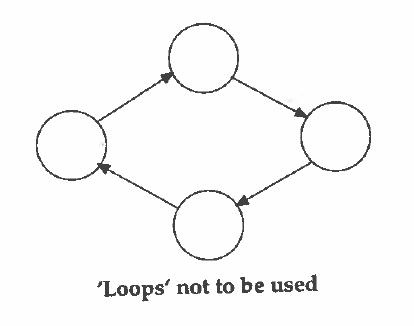
\includegraphics[width=0.3\linewidth]{324-c}
\caption{}
\label{fig:324-c}
\end{figure}
 \newpage


%- 324 


% 22 Network analysis — introduction and terminology 
	\item[(f)]  All activities must be tied into the network i.e. they must contribute to the progres-
sion or be discarded as irrelevant. Activities which do not link into the overall project 
are termed 'danglers'. 
\end{itemize}
\begin{figure}[h!]
\centering
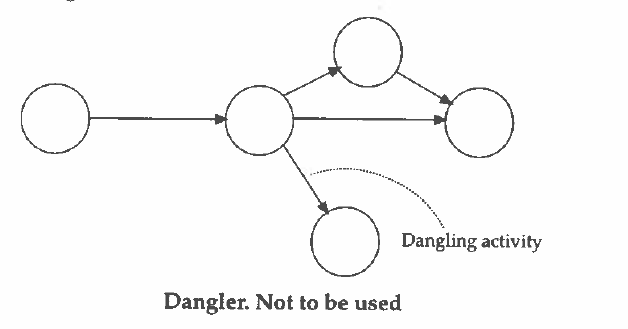
\includegraphics[width=0.4\linewidth]{325-a}
\caption{}
\label{fig:325-a}
\end{figure}

\subsection*{Conventions for drawing networks }
In addition to the Rules, which must not be violated, certain 
conventions are usually observed and for the sake of uniformity and easier communica-
tion students are recommended to follow the normal conventions. 
\begin{itemize}
	\item[(a)] Networks proceed from left to right. 
	\item[(b)]  Networks are not drawn to scale i.e. the length of the arrow does not represent time 
elapsed. 
	\item[(c)]  Arrows need not be drawn in the horizontal plane but unless it is totally unavoidable 
they should proceed from left to right. 
	\item[(d)]  If there are not already numbered, events or nodes should be progressively 
numbered from left to right. Simple networks may have events numbered in simple 
numeric progression i.e. 0, 1, 2, 3 etc but larger, more realistic networks may be 
numbered in 'fives' i.e. 0, 5, 10, 15 etc or 'tens' i.e. 0, 10, 20, 30 etc. This enables addi-
tional activities to be inserted subsequently without affecting the numbering 
sequence of the whole project. 
\end{itemize}
\subsection*{Activity identification }
Activities may be identified in several ways and students should familiarise themselves 
with the various methods so that unfamiliar presentation does not cause confusion. 
Typical of the methods to be found include: 
\begin{itemize}
\item[(a)]  Shortened description of the job e.g. plaster wall, order timber etc. 
\item[(b)]  Alphabetic or numeric code. e.g. A, B, C etc. or 100, 101, 108 etc. 
\item[(c)]  Identification by the tail and head event numbers e.g. 1-2, 2-3, 2-5 etc. 
\end{itemize}
\subsection*{Dummy activities }
It will be recalled that a dummy activity is one that does not consume time or resources 
but merely shows a logical relationship. It is shown on a network by a dotted arrow. 
Dummy example. Assume that part of the network involves a car arriving at a service 
station during which two independent activities take place, filling with petrol (A) and 
topping up with oil (B). 
%- 325 


%=================%
% 22 Network analysis — introduction and terminology 
% Page 326
This could be shown thus (incorrectly) 
\begin{figure}[h!]
\centering

\includegraphics[width=0.4\linewidth]{326-a}
\caption{}
\label{fig:326-a}
\end{figure}

NB. This is wrong because it contravenes rule (b) para 5. 
By the use of a dummy activity it could be shown thus (correctly) 
\begin{figure}[h!]
\centering
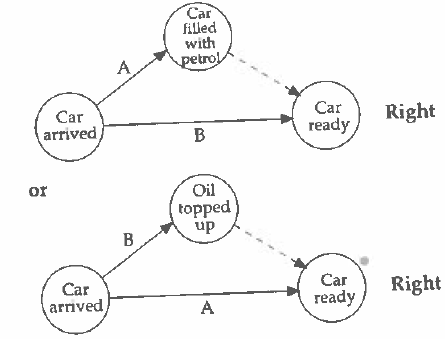
\includegraphics[width=0.47\linewidth]{326-b}
\caption{}
\label{fig:326-b}
\end{figure}

Further dummy example. Assume that part of a network involves a man lighting a ciga-
rette. The activities involved, and their relationships are assumed to be as follows. 
Activity Preceding activity 
A — Remove cigarette from case (Relates to earlier part of network) 
C — Put cigarette case away A 
B — Strike match (Relates to earlier part of network) 
D — Light cigarette A, B 
The network could be drawn thus 
\begin{figure}[h!]
\centering
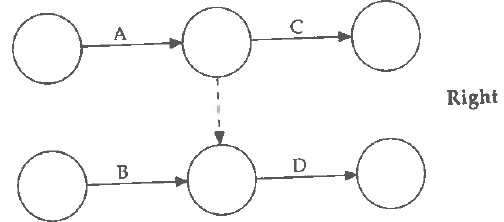
\includegraphics[width=0.4\linewidth]{326-c}
\caption{}
\label{fig:326-c}
\end{figure}

If the network had been drawn as follows it would have been incorrect. 
\begin{figure}[h!]
\centering
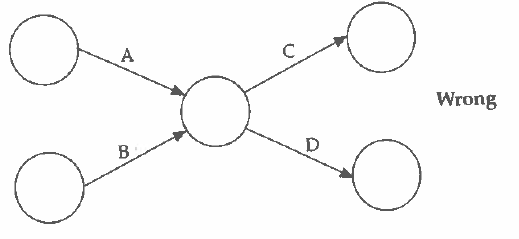
\includegraphics[width=0.4\linewidth]{326-d}
\caption{}
\label{fig:326-d}
\end{figure}


%==================%
% 22 Network analysis - introduction and terminology 
It is incorrect because it depicts that the cigarette case cannot be put away (C) until the 
match has been struck (B) which is incorrect according to the precedence rules given 
above. 
\subsection{Network example }
9. To summarise the material so far, a simple network example is given. Try to draw the 
network yourself and compare the logic of your network with the solution given. 
Project XXX Building a Boat 
man lighting a ciga-be as follows. 
,city 
of network) 
of network) 
Activity Preceding activity Activity description 
A Design Hull 
B Prepare Boat Shed 
C A Design Mast and Mast mount 
D A Obtain Hull 
E A Design Sails 
F C Obtain Mast Mount 
G C Obtain Mast 
H C Design Rigging 
B, D Prepare Hull 
K F, Fit Mast Mount to Hull 
L E, H, G, K Step Mast 
M E, H Obtain Sails and Rigging 
N L, M Fit Sails and Rigging Project XXX network 

Notes on solution given. 
a) The events have been numbered from 0, the start event, through to 8, the finish event. 
b) A dummy (4-6) was necessary because of the preceding activity requirements of 
activity L. If activities E, H had not been specified as preceding activity L, the dummy 
would not have been necessary. 
c) The shape of the network is unimportant but the logic must be correct. 

% - 327 
% - 22 Network analysis - introduction and terminology 

\subsection*{Summary} 10. a) Network analysis is used for the planning and control of large, complex projec b) Networks comprise activities (represented thus —÷) and events (represente 0). Activities consume time and resources, events are points in time. c) Networks have one start event and one end event. An event is not complete u activities leading into it are complete. d) The length of the arrows representing activities is not important because nel are not drawn to scale. e) Dummy activities (represented thus — -0.) are necessary to show logical re ships. They do not consume time or resources. They become necessary network is drawn. 
\subsection*{Points to note}
\begin{itemize}
	\item a) Network analysis is a popular type of examination question. b) Network analysis is an important management tool and in some industries civil engineering and construction, is used on a day by day basis. 
	\item c) Rarely does one draw a network in a neat, orderly fashion at the first at Accordingly it is is a useful examination technique to do a draft and copy tl neatly for the official answer. 
\end{itemize}
\subsection*{Self review questions} Numbers in brackets refer to paragraph numbers 1. What is Network Analysis?
\begin{enumerate}
	\item 
\end{enumerate} (2) 2 What are activities and events? (4) 3 What are the basic rules for drawing networks? (5) 4 Does the length of an activity arrow represent the time taken? (6) 5 What is a dummy activity? (8) 
Exercises with answers 1. Draw the network for the following problem. Activity Preceding activity 
1 -2,3,4 5 2 6 3 7 5 8 6 9 7, 8 10 3 11 4 12 9, 10, 11 2. Draw the network in question 1 except that Activity 8 is preceded by 6 and 2. 

% 328 
\newpage
%============%
\begin{figure}[h!]
\centering
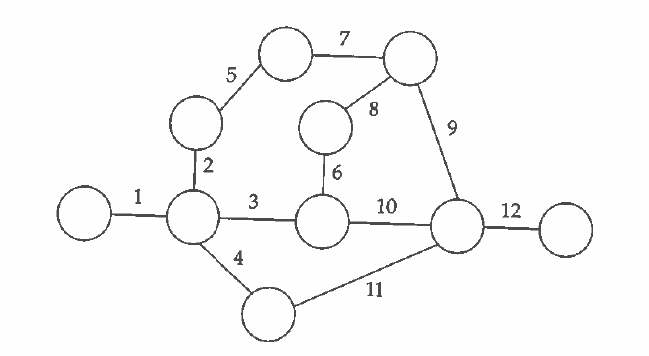
\includegraphics[width=0.4\linewidth]{329-A}
\caption{}
\label{fig:329-a}
\end{figure}
\begin{figure}[h!]
\centering
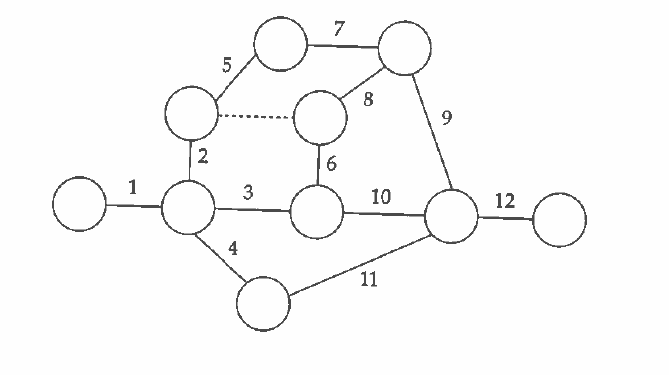
\includegraphics[width=0.4\linewidth]{329-b}
\caption{}
\label{fig:329-b}
\end{figure}

\end{document}
